\documentclass[11pt, a4paper]{article}

\usepackage{amsmath}
\usepackage{amsfonts} %Matheschriften
\usepackage{amssymb} %Mathesymbole
%\usepackage{mathptmx} % Einstellung für Schriften und Sonderzeichen in mathematischen Umgebungen
                        % ändert SChriftfont
\usepackage{wasysym} % Stellt diverse Sonderzeichen bereit
\usepackage{siunitx}
\usepackage{float}
\usepackage{microtype}
\usepackage{graphicx}


\usepackage[ngerman]{babel}
\addto\captionsngerman{%
 \renewcommand{\abstractname}{Abstract}}

\title{Versuch 2: Pendel}
\author{Jascha Fricker, Benedict Brouwer}

\begin{document}
    \maketitle

    

    \begin{abstract}
        In diesen beiden Versuchsaufbauten werden verschiedene Pendel untersucht. Zum einen wird mit
        einem Reversionspendel die Erdbeschleunigung $g$ gemessen, zum anderen werden zwei mit einer Feder
        gekoppelte Pendel untersucht und mit den Messwerten u.a. die Federkonstante berechnet.
    \end{abstract}

    \tableofcontents

    \section{Reversionspendel}

    \subsection{Experimenteller Aufbau und Theorie}

    Ein Reversionspendel hat zwei Aufhängepunkte und zwei Massen, die alle auf einer Geraden liegen.
    Dabei kann ein Masse verschoben werden.
    Es gibt zwei Positionen des verschiebbaren Gewichts, an dem die Periode der Schwingung an beiden
    Aufhängepunkten gleich ist. Für ein Reversionspendel in dieser Konfiguration ist die Periode
    \begin{align}
        \tau^2 = 4\pi^2 \cdot \frac{l_r}{g}
    \end{align}
    (Herleitung siehe \cite[Abschitt 1.3]{pen}). Daraus ist ersichtlich, dass, wenn dieser Fall eintritt, die Periodendauer unabängig von der Masse und des
    Trägheitsmoments ist. So kann mit der Periodendauer und dem Abstand der beiden Aufhängungspunkte $l_r$
    die Erdbeschleunigung ausgerechnet werden.
    Um diese besonderen Positionen der zweite Masse zu finden, wird im Experiment die Periodendauer
    mit der Masse an verschieden Positionen von beiden Aufhängungen gemessen,
    um dann mithilfe des Schnittpunkts der Ausgleichgeraden die gewünschten
    Punkte  zu bestimmen.



    \subsection{Ergebnisse}

    \begin{figure}[ht]
        \centering
        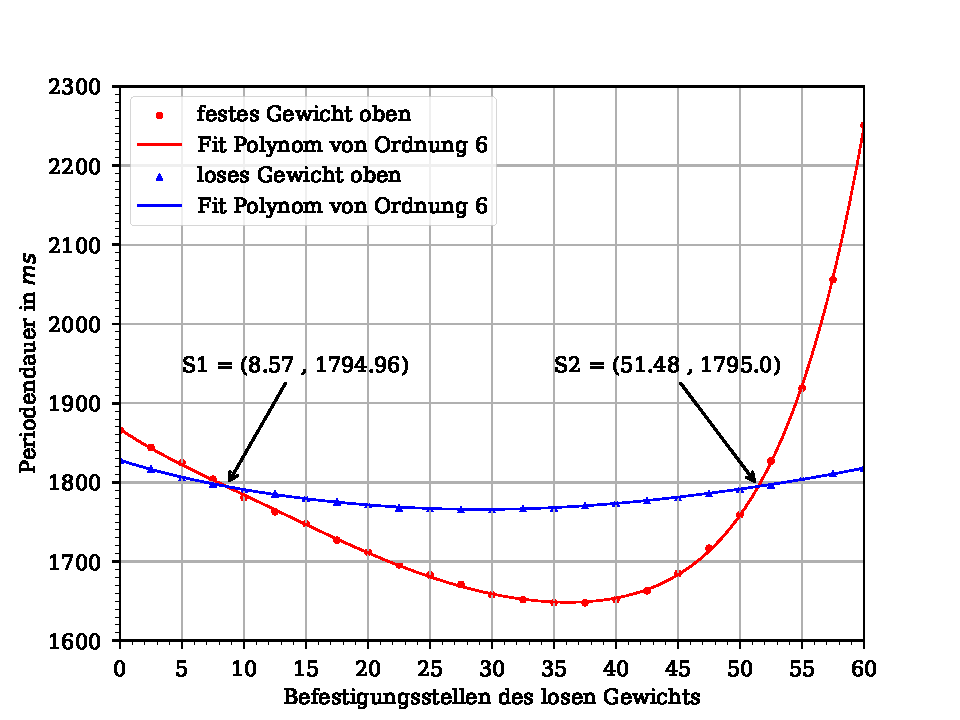
\includegraphics[width=120mm]{./Reversion_grob.pdf}

        \caption{Grobe Darstellung der Messdaten}
        \label{fig:revgrob}
    \end{figure}
    \begin{figure}[ht]
        \centering
        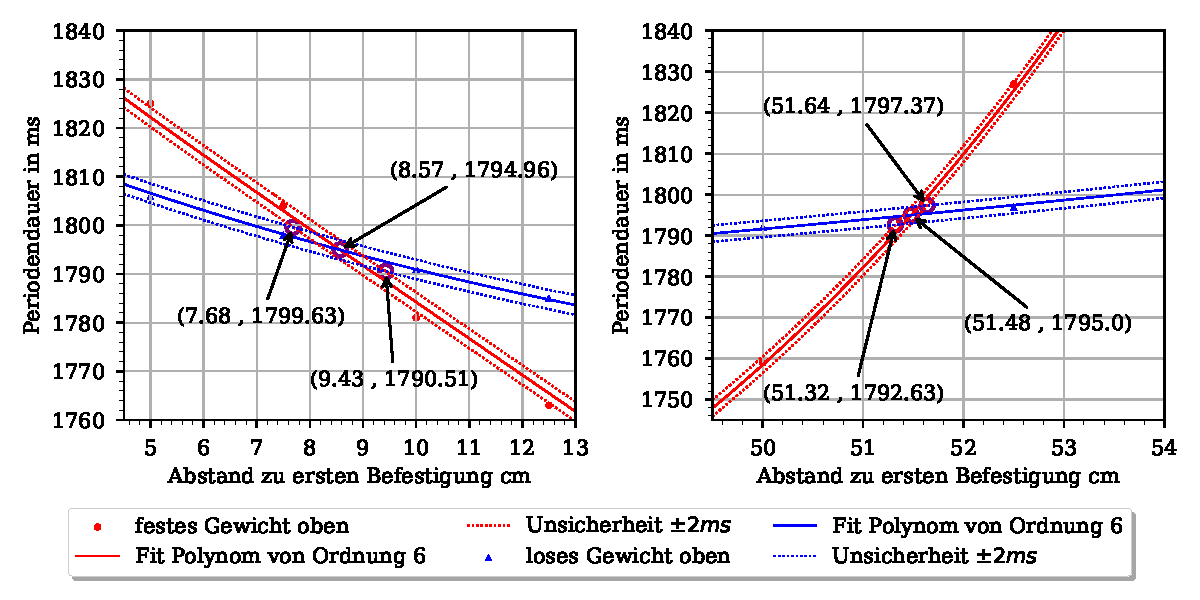
\includegraphics[width=120mm]{./Reversion_fein.pdf}

        \caption{Genauere Darstellung der Schnittpunkte}
        \label{fig:revfein1}
    \end{figure}

    Im Graphen \ref{fig:revgrob} wurde die Periodendauer abhängig vom Ort der zweiten Masse für beide Aufhängungspunkte dargestellt. 
    In den Graphen \ref{fig:revfein1} und ? können die beiden Schnittpunkte der Periodendauer der verschiedenen
    Aufhängungen nochmal näher gesehen werden. Für den Fehler der Zeitmessung
    wurden $2ms$ angenommen, da in den Messdaten eine maximale Abweichung von $1ms$ bei verschiedenen Messungen 
    der gleichen Periodendauer vorkam und die Lichtchranke selber eauch eine Genauigkeit von $1ms$ hat.
    Auf eine genaue Fehlerfortpflanzung wurde wegen der geringen Abweichung verzichtet, da wahrscheilich
    durch die Kleinwinkelnäherung viel größere Fehler entstehen.
    Beachtenswert ist, dass das Pendel einge Zeit brauch bis es sich "eingependelt" hat und konsistente Messwerte
    gemessen werden können. Der Abstand der beiden Aufhängungspunkte $l_r$ beträgt $800,00(25)cm$

    \begin{table}
        \centering
        \begin{tabular}{c|c|c}
            Schnittpunkt & 1 & 2 \\ \hline
            Periodendauer & & \\ \hline
            Erdbeschleunigung & &
        \end{tabular}
        \caption{Ergebisse}
        \label{ergrev}
    \end{table}

    Die in Tabelle \ref{ergrev} gedruckten Ergebnisse sind ? nah am Literaturwert von $g$. Diese liegt ?
    im Konfidenzintervall. Der gewichtete Mittelwert beträgt ?.

    \section{Gekoppelte Pendel}

    \subsection{Experimenteller Aufbau und Theorie}

    Gekoppelte Pendel sind zwei Pendel, die mit irgendwie miteinander gekoppelt sind. In diesem Fall sind
    zwei Pendel mit einer Feder auf einer veräanderbaren Höhe verbunden. 

    \subsection{Ergebnisse}

    \bibliographystyle{plain}
    \bibliography{literature}


\end{document}